\documentclass[12pt]{article}
\usepackage{graphicx} % Required for inserting images
\usepackage[a4paper,top=50pt,bottom=70pt,left=30pt,right=30pt]{geometry}
\usepackage[utf8]{inputenc}
\usepackage[OT1]{fontenc}
\usepackage[french]{babel}
\usepackage{fancyhdr}
\usepackage{lastpage}
\usepackage{changepage}


\title{S104 Rapport Final}
\author{Romain REN}
\date{\today}
\topmargin = -50pt

\begin{document}

    \pagestyle{fancy}
    \fancyhf{}
    \lhead{Projet S104}
    \chead{Romain REN, Marc ROUSSEL}
    \rhead{Rapport Final}
    \fancyfoot[R]{Page \thepage/\pageref{LastPage}}
    
    \begin{titlepage}
    \vbox{ }

    \begin{center}
        
\includegraphics[width=1\textwidth]{logo-iutorsay.png}\\[4cm]
        \textsc{\Large Création d'une base de données}\\[0.7cm]

        \noindent\makebox[\linewidth]{\rule{.7\paperwidth}{.6pt}}\\[0.7cm]
        { \huge \bfseries S104}\\[0.25cm]
        \noindent\makebox[\linewidth]{\rule{.7\paperwidth}{.6pt}}\\[0.7cm]
        \large{2022 - 2023}\\[1.2cm]
        \vfill
        \large
        Romain REN, Marc ROUSSEL

        {\large 19 Janvier, 2023}
    \end{center}
    \end{titlepage}

    
    {\fontfamily{lmss}\selectfont
    \begin{adjustwidth}{20pt}{20pt}
    \tableofcontents
    \newpage

    
    \section{Entreprise - Clinique des Noriets}
    \subsection{Présentation de l'entreprise}
    
    L’entreprise que nous avons choisie d’étudier pour l’élaboration de notre projet est celle de la \textbf{Clinique des Noriets}, c’est une clinique spécialisé dans la maternité et aussi dans la gériatrie se situant à \textbf{Vitry-Sur-Seine}.\bigskip

    Elle est affiliée à \textbf{l’Hôpital Privé de Vitry} et est composée de deux bâtiments, un batiment principal où se trouve les patients hospitalisés et la plupart des bureaux des praticiens et de l’autre côté un laboratoire qui s’occupe des analyses, tests PCR, etc.
    
    \subsection{Pourquoi cette entreprise ?}
    Nous avons décidé de choisir cette entreprise pour le projet car nous nous voulions proposer un travail plus qualitatif et complet.\bigskip
    
    La clinique étant assez complexe, il y avait plus d’informations à prendre en compte sachant que c’est aussi une entreprise dans le domaine médical, ce qui permet de concevoir dans un but réelle : moderniser les systèmes informatiques.\bigskip
    
    En choisissant cette entreprise, nous avons eu un réel aperçu de la complexité d’un système de données.
    
    \subsection{Organisation de l'entreprise}
    
    Les patients viennent à l’accueil de la clinique pour s’inscrire à la maternité ou à d’autres services, une date d’admission est fixée, lors de la date ou plus tôt (ce sont des prévisions de grossesses donc ça peut arriver plus tôt) les patients sont admis dans l’établissement, ils y passent un certain temps selon leurs besoins, de 3 à 7 jours, ils ont différentes prestations payantes(la télévision, le wifi, etc.) qu’ils peuvent demander et à la fin du séjour, ils règlent la chambre et les différentes prestations, les factures et dossiers sont envoyés aux facturières qui les clôturent si tout est bon ou sinon les renvoient pour les faire compléter ou si des paiements sont manquants, elles envoient les factures à l’adresse des patientes.\bigskip
    
    Donc d’abord, il y a une pré-admission pour pouvoir créer un dossier « patient » avec une date d’entrée de séjour prévue, il y a l’entrée réelle lors de l’admission, une date de sortie prévue selon l’avis des sages-femmes et une date de sortie réelle, il y a différentes prestations avec des prix différents, à la fin du séjour, la facture comportent toutes les prestations et le coût de la chambre et à la fin l’entièreté du dossier est envoyé à la facturière pour être clôturé. Il y a différents forfaits de chambre(normal, confort, premium).
    \newpage
    \section{Création de la base de données}
    \subsection{Modèle Conceptuelle de Données}
    Voici le modèle conceptuelle de données réalisé d'après l'organisation de la clinique :\bigskip\linebreak
    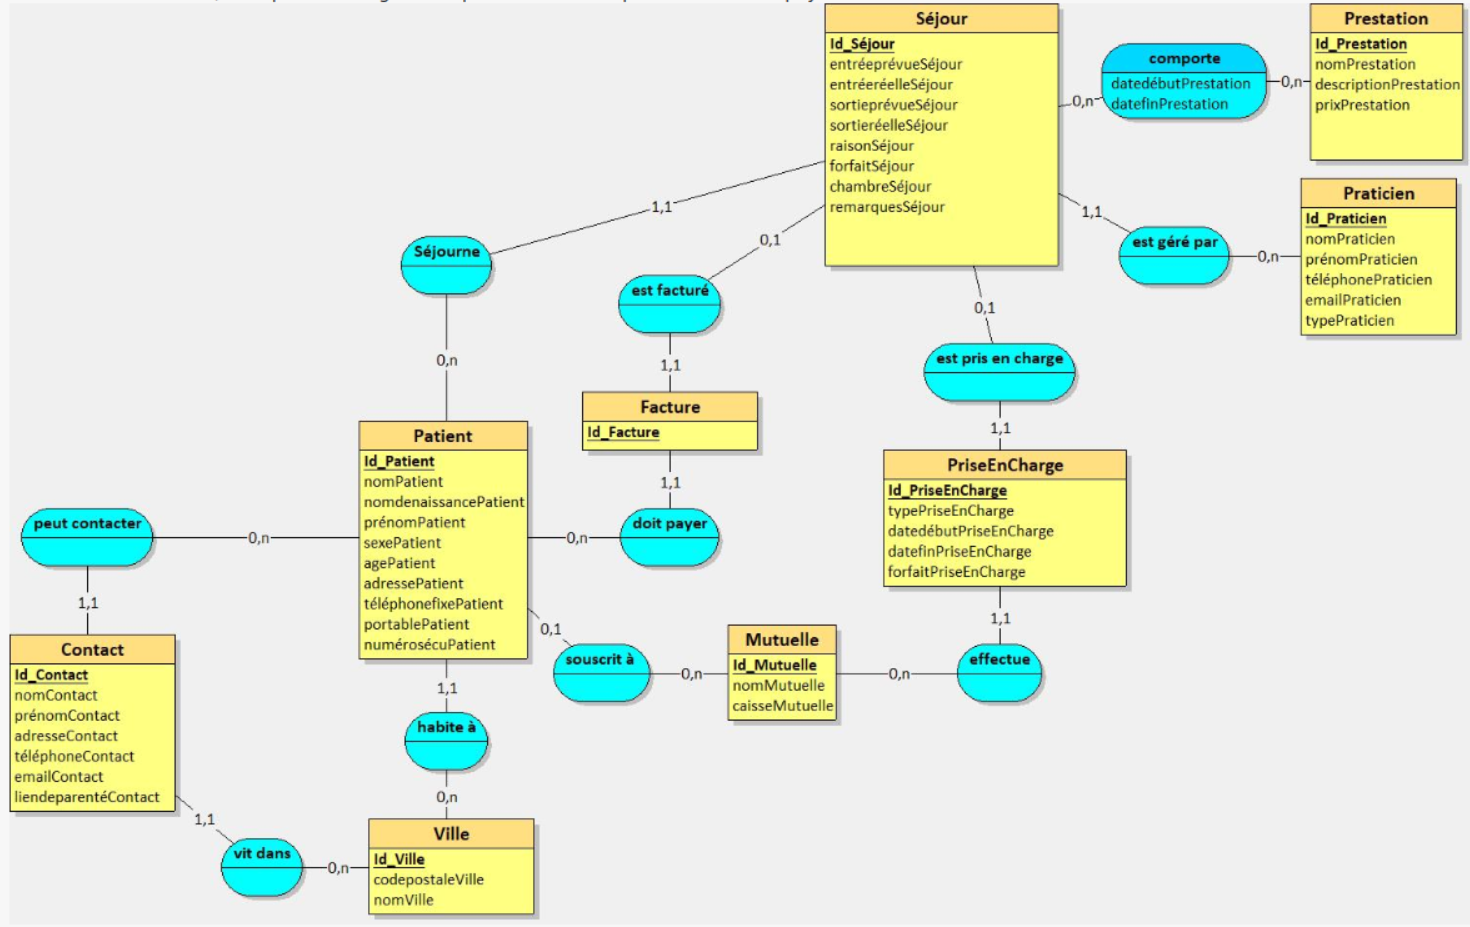
\includegraphics[width=0.9\textwidth]{MCD.png}\\[4cm]
    \newpage
    \subsection{Schéma relationnel}
    Voici le schéma relationnel réalisé d'après le modèle conceptuel de données :\bigskip\linebreak
    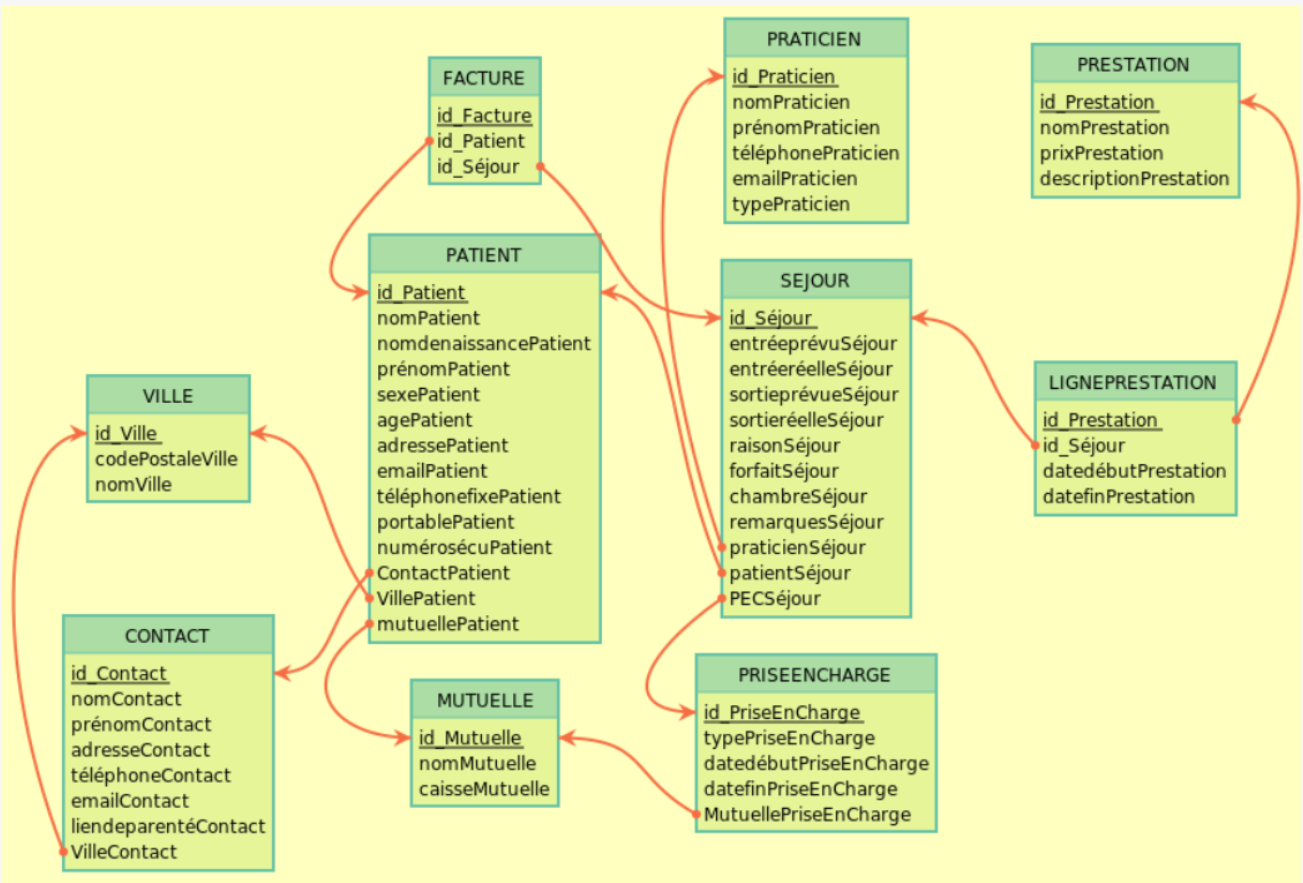
\includegraphics[width=0.9\textwidth]{SR.png}\\[4cm]
    \newpage
    \subsection{Dictionnaire de données}
    Voici le dictionnaire de données de la base de données de la clinique :\bigskip\linebreak
    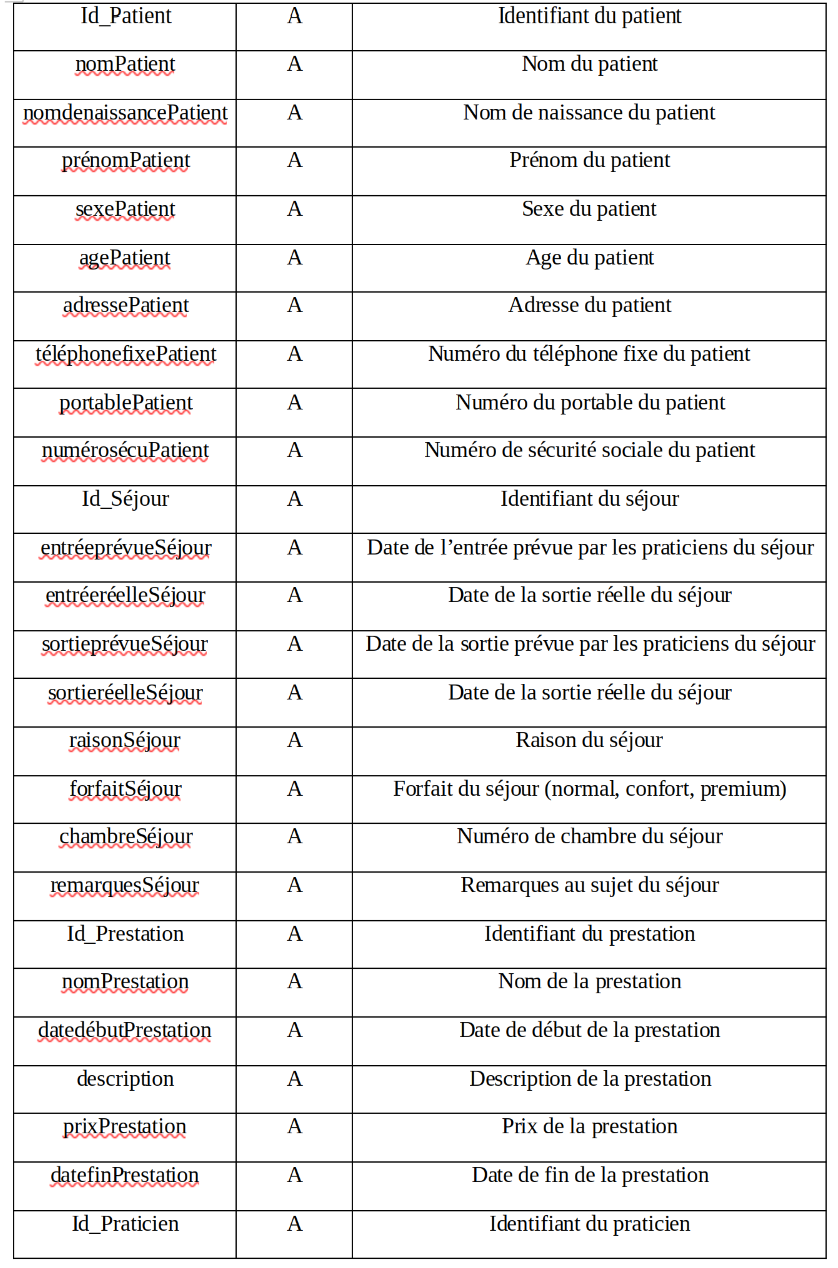
\includegraphics[width=0.82\textwidth]{DD1.png}\\[4cm]
    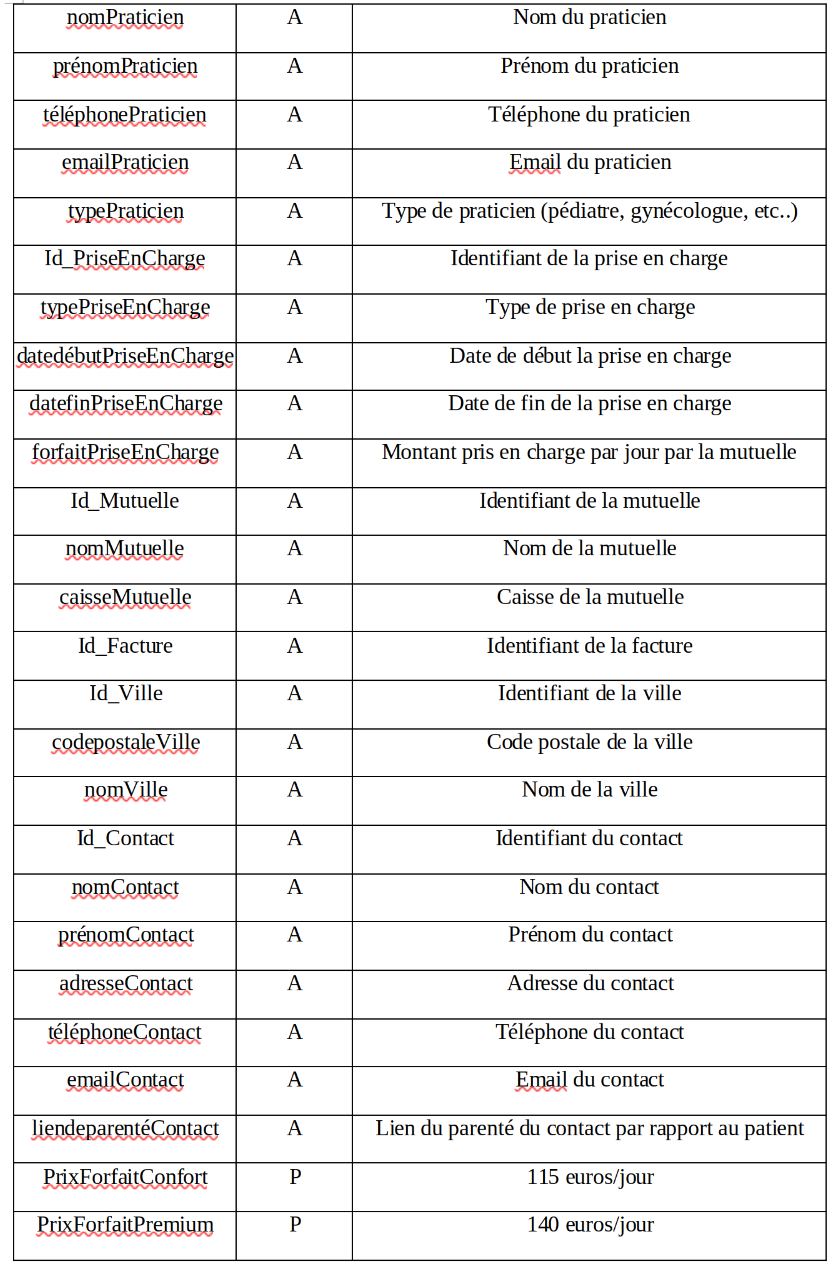
\includegraphics[width=0.82\textwidth]{DD2.png}\\[4cm]
    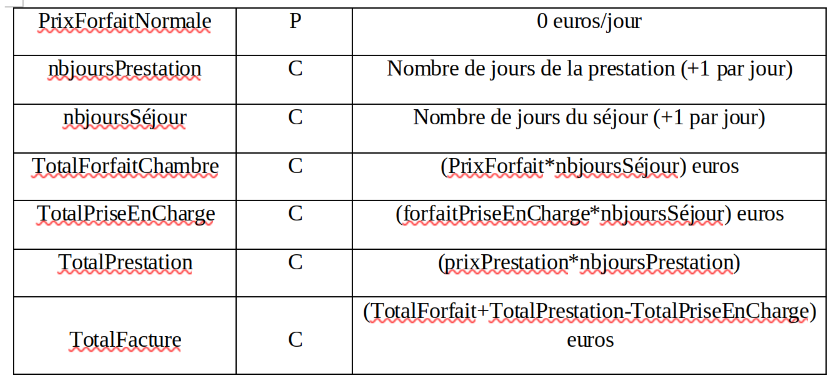
\includegraphics[width=0.82\textwidth]{DD3.png}\\[4cm]
    \newpage
    \subsection{Contraintes non modélisables}
    PECSéjour signifie PriseEnChargeSéjour (pour le potentiel remboursement du séjour pris en charge par la mutuelle) et elle peut être nulle mais pas négatif (si la mutuelle refuse la prise en charge).\bigskip

    forfaitSéjour correspond au type de séjour qu'ils ont demandés (Premium, confort ou double) et peut être nul si le type est double (une chambre partagée par deux personnes).\bigskip
    
    agePatient peut être positif ou nul (si c'est un bébé).\bigskip

    L'attribut prixPrestation ne peut pas être négatif et nulle (c'est un prix).\bigskip
    
    emailPraticien,emailPatient et emailContact sont au format email (avec un @ et finissant par '.fr','.com',etc ).\bigskip
    
    numerosécuPatient est un nombre de 13 chiffres commençant par 1 ou 2 et doit correspondre à un numéro existant.\bigskip
    
    dateFinPrestation doit venir après dateDébutPrestation comme les autres dates (entréeprévuSéjour, entréeréelleSéjour, sortieprévueSéjour, sortieréelleSéjour).\bigskip
    sexePatient ne peut être que féminin ou masculin (aucun autre genre accepté).\bigskip
    codePostaleVille est un nombre à 5 chiffres, les numéros de téléphone (téléphonefixePatient, portablePatient, téléphonePraticien, téléphoneContact) sont à 10 chiffres.\bigskip
    
    chambreSéjour doit être une vraie chambre correspondant à des chiffres et des lettres (211F, c'est une chambre double, ça indique la chambre à l'étage 2 numéro 11 du côté de la fenêtre)
    \end{adjustwidth}
    }
\end{document}